
% This LaTeX was auto-generated from an M-file by MATLAB.
% To make changes, update the M-file and republish this document.

\documentclass{article}
\usepackage{graphicx}
\usepackage{color}

\sloppy
\definecolor{lightgray}{gray}{0.5}
\setlength{\parindent}{0pt}

\begin{document}

    
    
\section*{testG}

\begin{par}
Example for algorithm testG. Algorithm is usefull only for testing QWTB toolbox. It calculates maximal and minimal value of the record. GUF is calculated by wrapper.
\end{par} \vspace{1em}
\begin{par}
See also \texttt{qwtb}
\end{par} \vspace{1em}

\subsection*{Contents}

\begin{itemize}
\setlength{\itemsep}{-1ex}
   \item Generate sample data
   \item Call algorithm
   \item Plot results
\end{itemize}


\subsection*{Generate sample data}

\begin{par}
Two quantities are prepared: \texttt{t} and \texttt{y}.
\end{par} \vspace{1em}
\begin{verbatim}
t.v = [1:20];
y.v = [1:14 13:-1:8];
\end{verbatim}
\begin{par}
All uncertainties are set to 1.
\end{par} \vspace{1em}
\begin{verbatim}
t.u = t.v.*0 + 1;
y.u = y.v.*0 + 1;
\end{verbatim}
\begin{par}
Set degrees of freedom.
\end{par} \vspace{1em}
\begin{verbatim}
t.d = t.v.*0 + 60;
y.d = y.v.*0 + 9;
\end{verbatim}
\begin{par}
Quantities are put into data input structure \texttt{DI}.
\end{par} \vspace{1em}
\begin{verbatim}
DI.t = t;
DI.y = y;
\end{verbatim}
\begin{par}
Create calculation settings \texttt{CS} and set uncertainty calculation method to GUM uncertainty framework.
\end{par} \vspace{1em}
\begin{verbatim}
CS = [];
CS.unc = 'guf';
\end{verbatim}


\subsection*{Call algorithm}

\begin{par}
Use QWTB to apply algorithm \texttt{testG} to data \texttt{DI} with calculation settings \texttt{CS}.
\end{par} \vspace{1em}
\begin{verbatim}
DO = qwtb('testG', DI, CS);
\end{verbatim}

        \color{lightgray} \begin{verbatim}QWTB: default correlation matrix generated for quantity `t`
QWTB: default correlation matrix generated for quantity `y`
QWTB: uncertainty calculation by means of wrapper or algorithm
\end{verbatim} \color{black}
    

\subsection*{Plot results}

\begin{par}
Plot input data and calculated maximal and minimal values as a red and green lines with uncertainties represented by dashed lines.
\end{par} \vspace{1em}
\begin{verbatim}
figure
hold on
errorbar(DI.t.v, DI.y.v, DI.y.u, 'xb')
plot([DI.t.v(1) DI.t.v(end)], [DO.max.v DO.max.v], '-r', 'linewidth', 3)
plot([DI.t.v(1) DI.t.v(end)], [DO.max.v - DO.max.u DO.max.v - DO.max.u], '--r', 'linewidth', 3)
plot([DI.t.v(1) DI.t.v(end)], [DO.min.v DO.min.v], '-g', 'linewidth', 3)
plot([DI.t.v(1) DI.t.v(end)], [DO.min.v - DO.min.u DO.min.v - DO.min.u], '--g', 'linewidth', 3)
plot([DI.t.v(1) DI.t.v(end)], [DO.max.v + DO.max.u DO.max.v + DO.max.u], '--r', 'linewidth', 3)
plot([DI.t.v(1) DI.t.v(end)], [DO.min.v + DO.min.u DO.min.v + DO.min.u], '--g', 'linewidth', 3)
legend('original data (DI.t.v, DI.y.v)', 'line at maximum value (DO.max.v)', 'uncertainty',  'line at minimum value (DO.min.v)', 'uncertainty', 'location', 'southoutside')
xlabel('quantity t')
ylabel('quantity y')
title('input data and results of testG algorithm')
hold off
\end{verbatim}

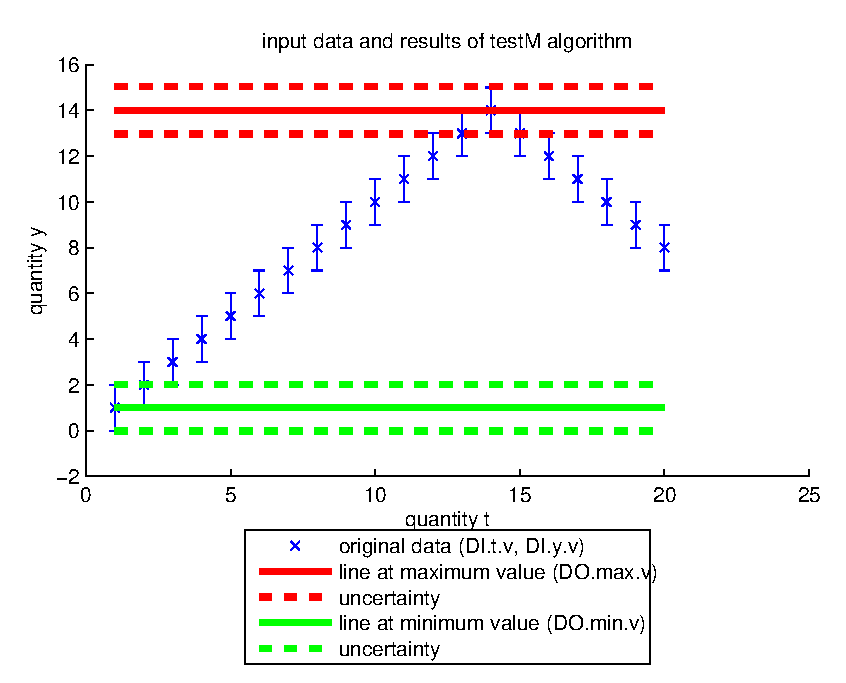
\includegraphics [width=4in]{alg_example_01.eps}



\end{document}
    
